%!TeX root = main.tex
%!TeX spellcheck = fr-FR
% Nicolas Castel PhD thesis -- (C) 2023

\documentclass[thesis]{subfiles}

\begin{document}

\begin{otherlanguage}{french}

\renewcommand{\thesection}{\arabic{section}}
\renewcommand{\thesubsection}{\arabic{section}.\arabic{subsection}}
\renewcommand{\thefigure}{R\arabic{figure}}
\setcounter{figure}{0}
\titlecontents{section}[4.8em]{\addvspace{0.1em}}{\contentslabel{2.2em}}{}{\titlerule*[1pc]{.}\contentspage}[]

\chapter*{Résumé en français}
\startcontents[chapters]
\printpartialtoc

\section*{Introduction}

Les procédés industriels de séparation des gaz sont utilisés dans diverses industries, telles que la chimie, la santé, l'agriculture et l'alimentation, pour fournir des réactifs purifiés et des gaz inertes. Ces procédés sont également utilisés pour atténuer les effets négatifs de certaines activités industrielles sur l'environnement, comme la capture du dioxyde de carbone dans les usines de production de béton ou d'acier ou encore le piégeage de composés radioactifs volatils des usines de retraitement des combustibles nucléaires. Différentes petites molécules comme le diazote, le dioxygène, le dioxyde de carbone, le dihydrogène, le méthane, le protoxyde d'azote ou les gaz rares sont ainsi séparées, purifiées puis stockées. Cette thèse se concentre sur la séparation xénon/krypton communément utilisée pour extraire ces gaz de l'atmosphère, mais aussi de l'industrie du nucléaire qui constitue une source bien plus abondante de xénon et de krypton.

Les procédés industriels de séparation Xe/Kr sont encore bien souvent basés sur la distillation cryogénique de l'air ambiant, ce qui requiert beaucoup d'énergie, une infrastructure complexe et un contrôle minutieux des risques. On peut par exemple évoquer les récents accidents d'exploitation d'usine de séparation de gaz (1997) qui ont été causés notamment par la réaction d'hydrocarbures de l'environnement avec l'oxygène liquéfié de l'usine. Pour éviter les problèmes de sécurité et de coûts importants, de nombreux chercheurs s'attèlent à développer des méthodes de séparation industrielle basées sur l'adsorption dans des matériaux nanoporeux. Ces matériaux nanoporeux sont constitués de pores à l'échelle nanoscopique qui offrent une large surface aux molécules pour y interagir puis s'adsorber. Des procédés industriels basés sur cette technologie existent déjà, ils utilisent notamment le \emph{pressure swing adsorption} (PSA) qui consiste à remplir les pores d'un mélange de gaz à haute pression, puis de récupérer un gaz ainsi purifié. En effet, les pores du matériau permettent l'adsorption préférentielle d'une molécule par rapport aux autres ce qui permet d'augmenter la teneur en une certaine molécule du mélange sortant. En répétant ce procédé, on peut ainsi séparer les différentes molécules d'un gaz. Dans le cadre de ma thèse, le xénon étant chimiquement proche du krypton, la purification par ce procédé reste un défi majeur. Certains prototypes industriels ont déjà été imaginés, mais la recherche d'un matériau pour effectuer au mieux cette tâche reste aujourd'hui une question ouverte. 

Pour développer un procédé viable, il faut donc choisir avec soin les matériaux que l'on utilise dans ces dispositifs industriels. La recherche se focalise aujourd'hui sur la conception de matériaux toujours plus sélectifs en se basant sur des intuitions chimiques construites au fil des études. Afin d'éviter les expériences coûteuses pour tester tous les matériaux, les criblages computationnels sont de plus en plus utilisés. Ces criblages ou \emph{screenings} en anglais permettent de passer en revue de grandes quantités de structures afin d'en évaluer leur potentielle performance. Tout l'enjeu est donc de former une bonne synergie entre la conception minutieuse de matériaux et la recherche et évaluation rapide des matériaux via des méthodes informatiques. Du côté du traitement informatique des matériaux, les deux défis majeurs sont la génération de données fiables et diverses afin de couvrir le spectre des possibles et le développement de nouveaux outils pour l'évaluation rapidement et avec précision les performances de ces matériaux. 

La quantité de matériaux est potentiellement infinie, rien que pour les \emph{metal--organic frameworks} (MOFs) en anglais, plus de 90\,000 structures ont été synthétisées et 500\,000 ont été construits de manière digitale. Pour pouvoir évaluer tous ces matériaux, différentes stratégies ont été élaborées. Certains utilisent des criblages à plusieurs niveaux qui permettent de réduire au fur et à mesure les matériaux à évaluer avec des méthodes plus coûteuses, d'autres se basent sur des algorithmes d'apprentissage statistique. Cependant, peu d'études se focalisent sur les outils de calcul, en eux-mêmes, qui sont souvent davantage adaptés à des calculs sur des structures uniques plutôt que pour être déployés sur des centaines de milliers de structures. Cette thèse s'emploie donc à développer des outils pour accélérer les procédés de criblages actuels tout en travaillant sur la précision des évaluations de performance. Outre la sélectivité, d'autres variables revêtent une importance significative : la capacité d'adsorption du matériau, la cinétique et la thermodynamique derrière la régénération du matériau (c'est-à-dire en vider les pores). Pour cette raison, ma thèse étudie également les propriétés de transport du xénon et du krypton dans ces matériaux nanoporeux. 

\section*{\'Etude thermodynamique de la séparation Xe/Kr}

En premier lieu, mes travaux ont porté sur l'analyse poussée des corrélations qu'il pouvait exister entre les différentes grandeurs thermodynamiques décrivant la séparation xénon/krypton. Pour cela, mes travaux se basent sur la base de données CoRE MOF 2019 pour comparer les différentes grandeurs thermodynamiques grâce à des analyses de corrélation. Différentes conditions de pression et de composition ont été étudiées et des explications physiques à l'échelle microscopique sont proposées pour comprendre l'origine des différences observées. 

Pour commencer, j'ai étudié les corrélations entre l'enthalpie et la sélectivité. Sur la figure~\ref{fgr:histo_H_resume}, l'enthalpie d'adsorption du xénon est assez bien corrélée au logarithme de la sélectivité à basse pression suggérant ainsi que l'affinité du xénon avec le matériau peut expliquer la sélectivité. Cette corrélation diminue cependant pour les matériaux moins sélectifs. Les matériaux les plus sélectifs ont en effet des pores dont la taille est très favorable à l'adsorption du xénon comme le suggèrent d'autres études. Pour des gaz nobles, seules les interactions de van der Waals jouent un rôle important, ainsi la taille des pores permettent d'expliquer en grande partie l'affinité comparée entre deux molécules de tailles différentes le xénon et le krypton. Ainsi, dans des matériaux avec de petits pores, les phénomènes sont dominés par les interactions entre les pores et l'adsorbat, c'est-à-dire par l'enthalpie. Alors que dans de larges pores, les effets entropiques jouent un rôle plus important.

\begin{figure}[h]
\begin{minipage}[t]{.43\textwidth}
\centering
  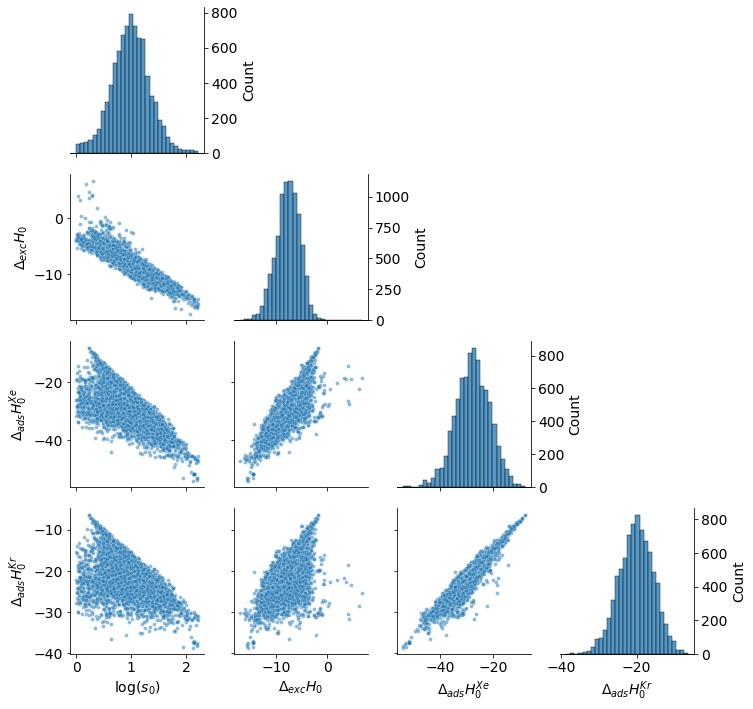
\includegraphics[width=\linewidth]{figures/2-thermo/Enthalpy_0_log.jpg}
  \caption{\small{\ Pour 8\,401 MOFs avec une sélectivité Xe/Kr favorable ($s\e{0} > 1$), pair-plots entre les différentes grandeurs $\log(s\e{0})$, $\Delta\e{exc}H\e{0}$, $\Delta\e{ads}H\ex{Xe}\e{0}$ et $\Delta\e{ads}H\ex{Kr}\e{0}$ (les enthalpies sont en \si{\kilo\joule\per\mol}) en dehors de la diagonale et la distribution de chaque grandeur sur la diagonale.}}\label{fgr:histo_H_resume}
\end{minipage}
\hfill
\begin{minipage}[t]{.5\textwidth}
\centering
  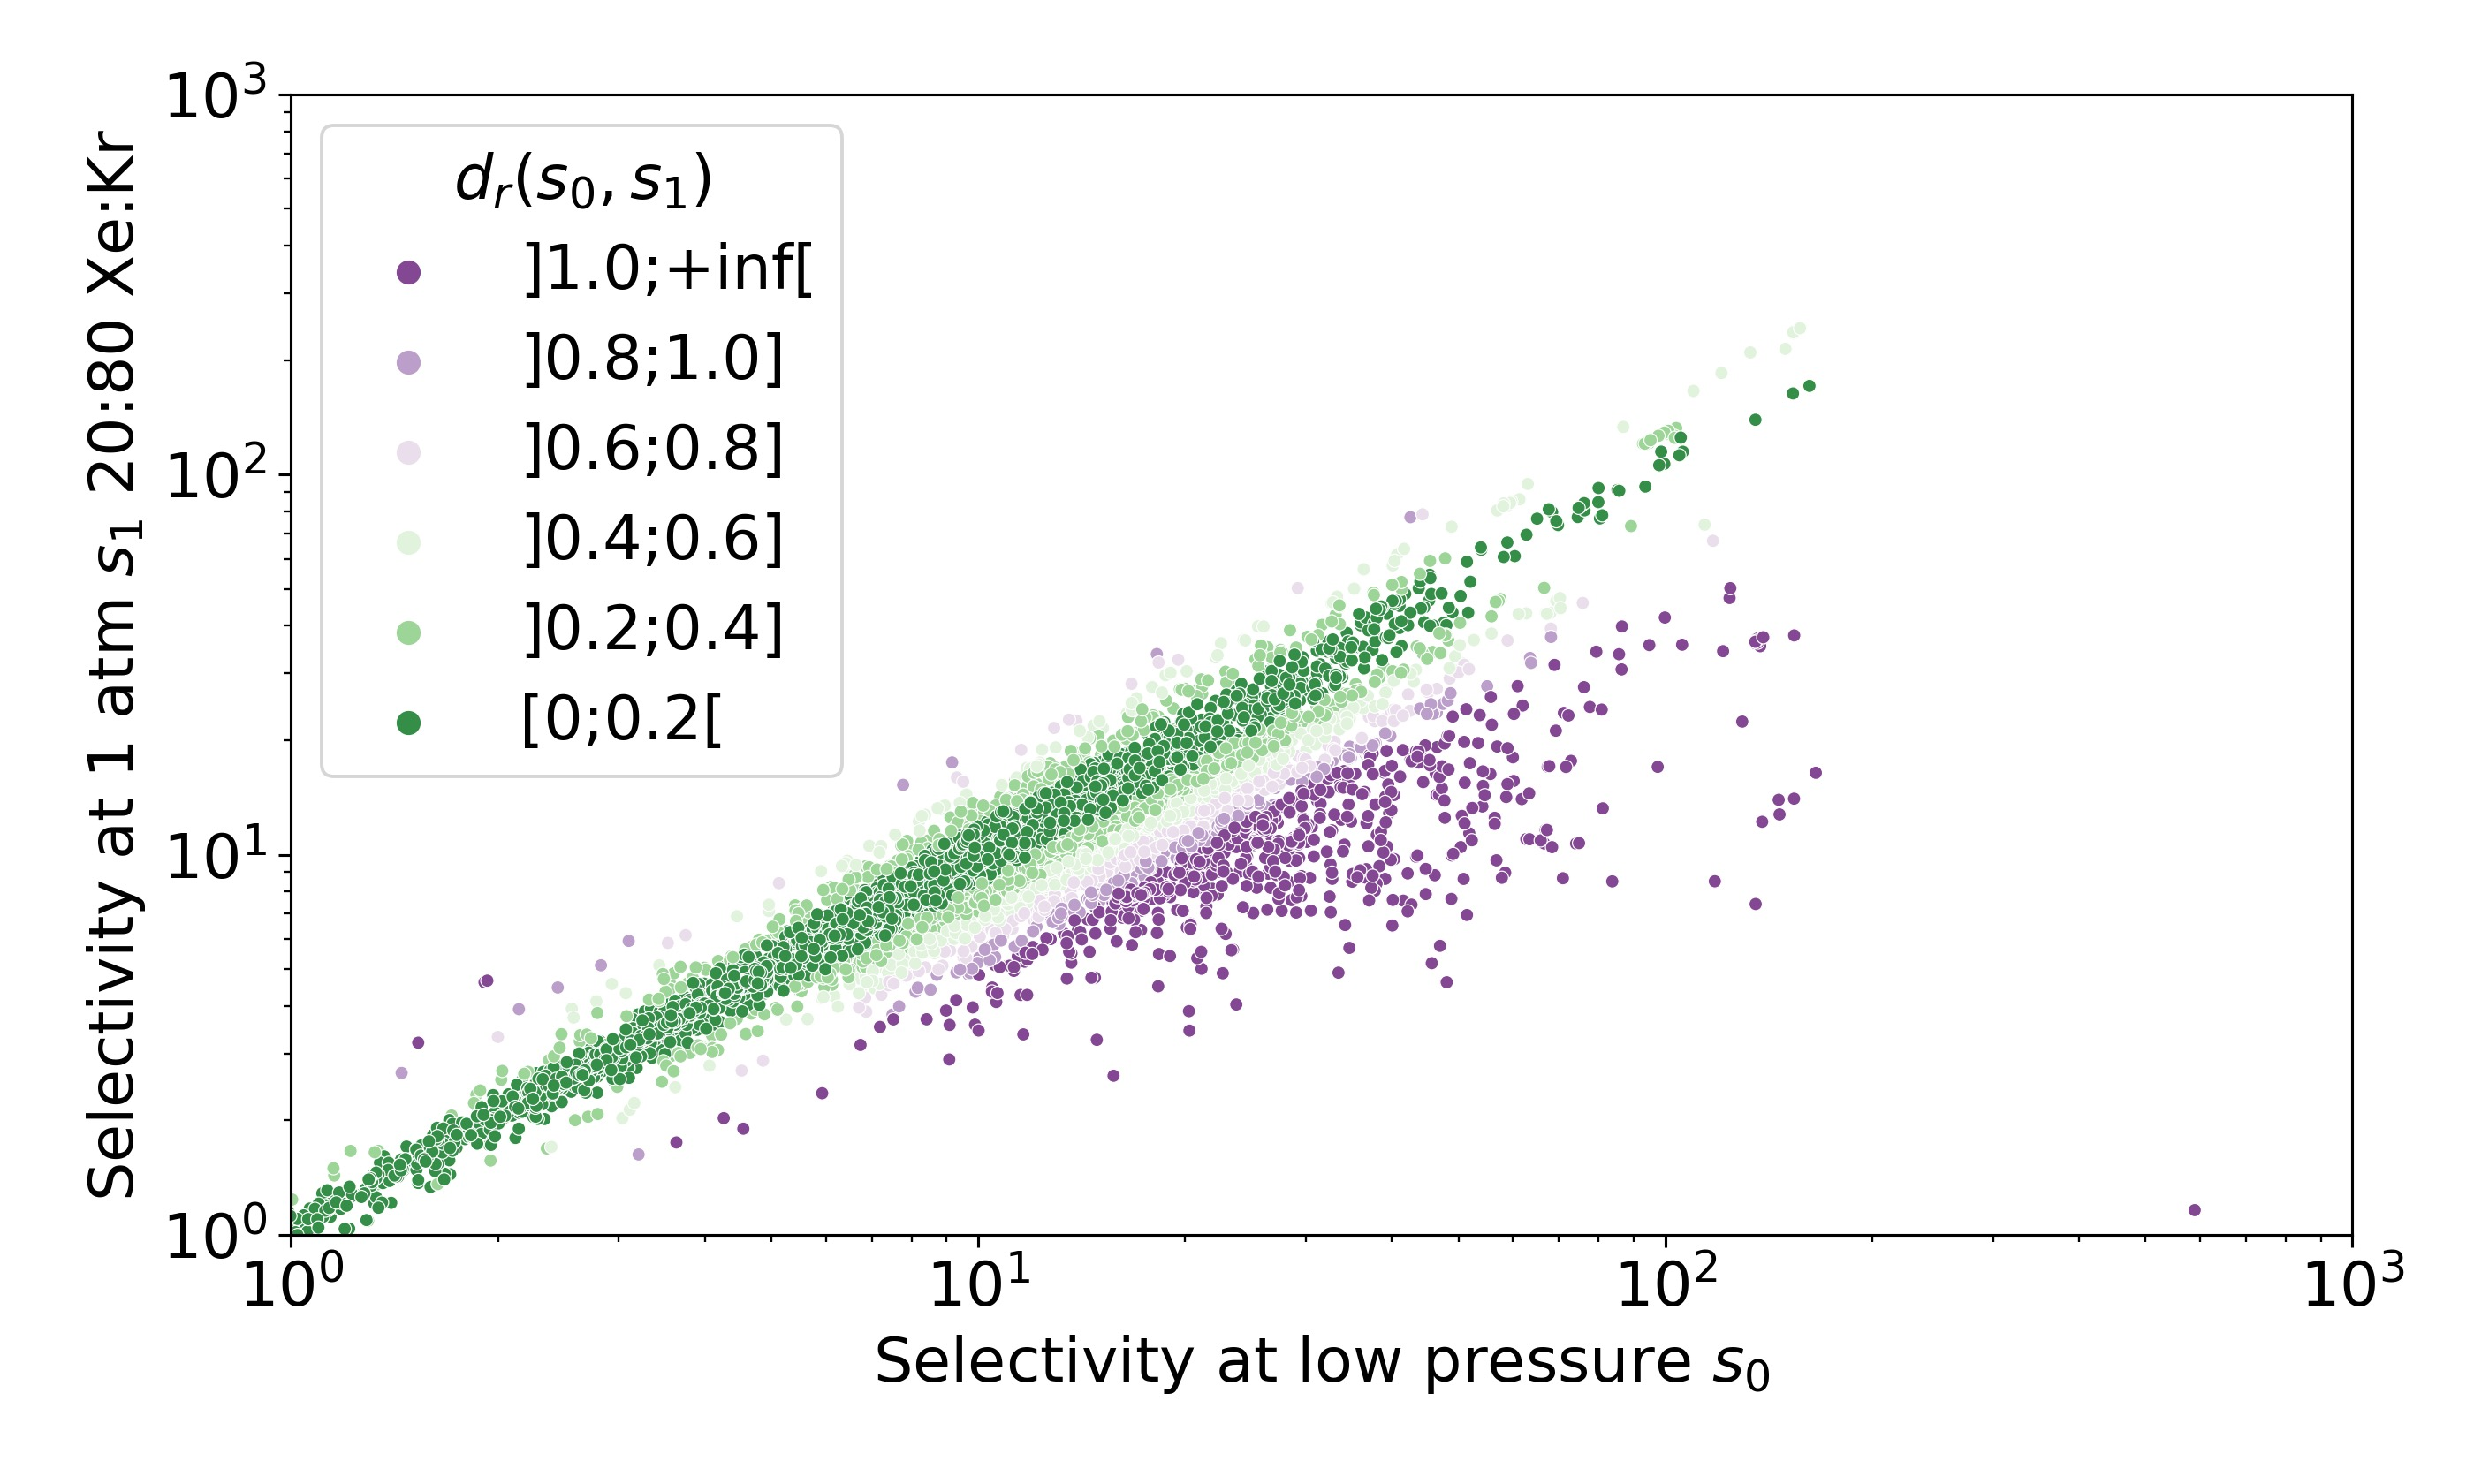
\includegraphics[width=\linewidth]{figures/2-thermo/s_0_vs_s_2080_overview_log.jpg}
  \caption{\small{\ Sélectivité à 1\,atm de pression en fonction de la sélectivité à basse pression pour une composition 20\pp{}80 Xe/Kr. Les points sont étiquetés selon la différence relative entre les deux sélectivités. Les points violets ont une grande différence relative entre les sélectivités. }}
  \label{fgr:overview_resume}
\end{minipage}
\end{figure}

D'autre part, nous observons sur la figure~\ref{fgr:histo_H_resume} que l'enthalpie d'échange est très bien corrélée à la sélectivité. Cela peut s'interpréter à l'aide de l'équation suivante $\Delta\e{exc}H= T\Delta\e{exc}S - RT\ln{s}$ dans le cas où $T\Delta\e{exc}S$ serait quasi constante. En effet, l'entropie joue le rôle de bruit d'un point de vue statistique ce qui est confirmé par d'autres figures au chapitre 2 de cette thèse, où l'on observe clairement l'absence totale de corrélation avec la sélectivité. Cette première figure nous renseigne ainsi sur le rôle prédominant de l'enthalpie d'échange pour expliquer la sélectivité observée. 

La figure~\ref{fgr:overview_resume} quant à elle met en évidence la chute de la sélectivité de certains matériaux lorsque l'on passe de la basse pression à la pression ambiante. Cette différence de sélectivité est étudiée à l'aide de l'enthalpie et l'entropie d'échange. Et nous remarquons à nouveau que ce changement de sélectivité est en grande partie expliqué par une augmentation de l'enthalpie d'échange pour ces structures. L'entropie joue encore un rôle relativement mineur sur ce phénomène. L'étude des données thermodynamiques sur un ensemble de 9\,668 structures nous suggère que l'enthalpie d'échange définie précédemment permet d'expliquer en grande partie les tendances des sélectivités thermodynamiques à haute et basse pression. La séparation xénon/krypton est donc dominée par des effets enthalpiques. 

Pour mettre en évidence les phénomènes physiques à l'origine de la chute de sélectivité pour certains matériaux, nous allons présenter dans ce résumé une structure problématique en particulier pour illustrer les caractéristiques de la structure. 
Dans ce matériau, il n'y a pas qu'un seul type de site d'adsorption ni un seul canal unidirectionnel. Le matériau WOJJOV (figure~\ref{WOJJOV_resume}) est un exemple de structure contenant deux types de pores comme on peut le voir sur la représentation graphique et ce qui est confirmé par la validité d'un modèle à 2 sites pour décrire les isothermes corps pur. Le premier type de type est plus petit et a une taille parfaite pour adsorber le xénon. C'est pourquoi, à basse pression la sélectivité calculée est très élevée $s_0=146$. Lorsqu'on augmente la pression, les sites plus larges commencent à être occupés. Or ces sites plus larges sont moins sélectifs du fait de leur taille. C'est pourquoi la sélectivité diminue grandement et passe à $s_1=14$ à pression ambiante. D'autres structures ayant un système plus complexe de canaux baissent également en sélectivité avec la pression.

\begin{figure*}[h]
\centering
  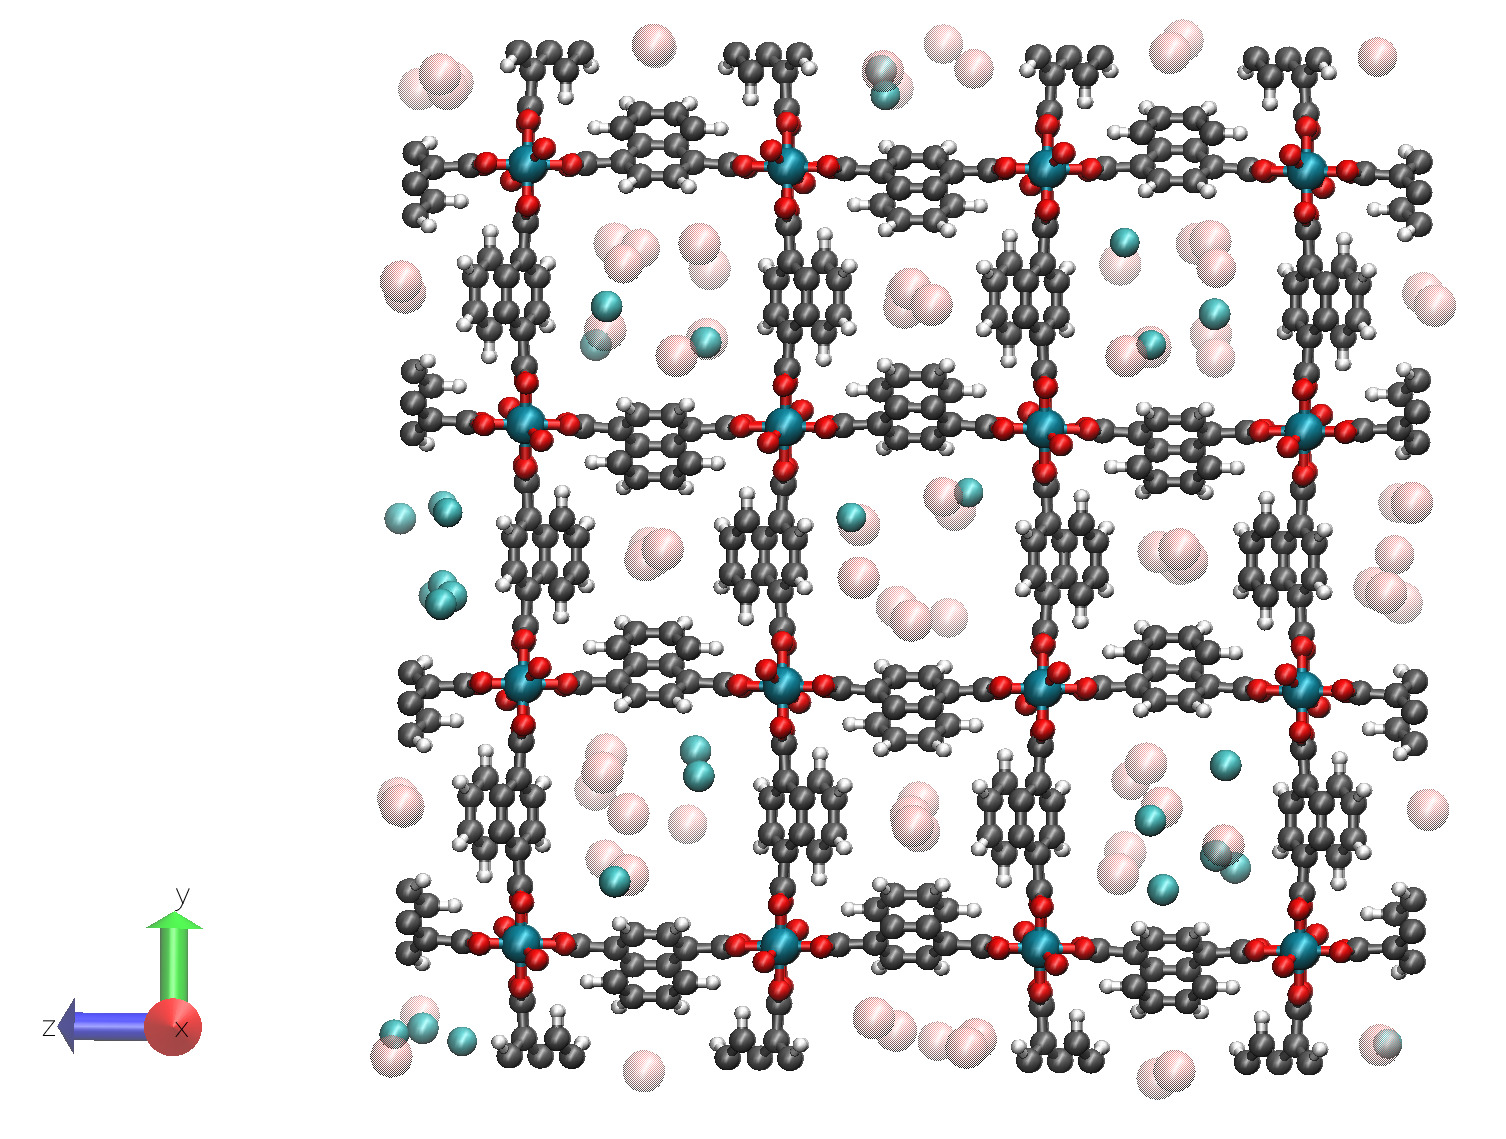
\includegraphics[width=0.4\textwidth]{figures/2-thermo/WOJJOV_clean.jpg}
  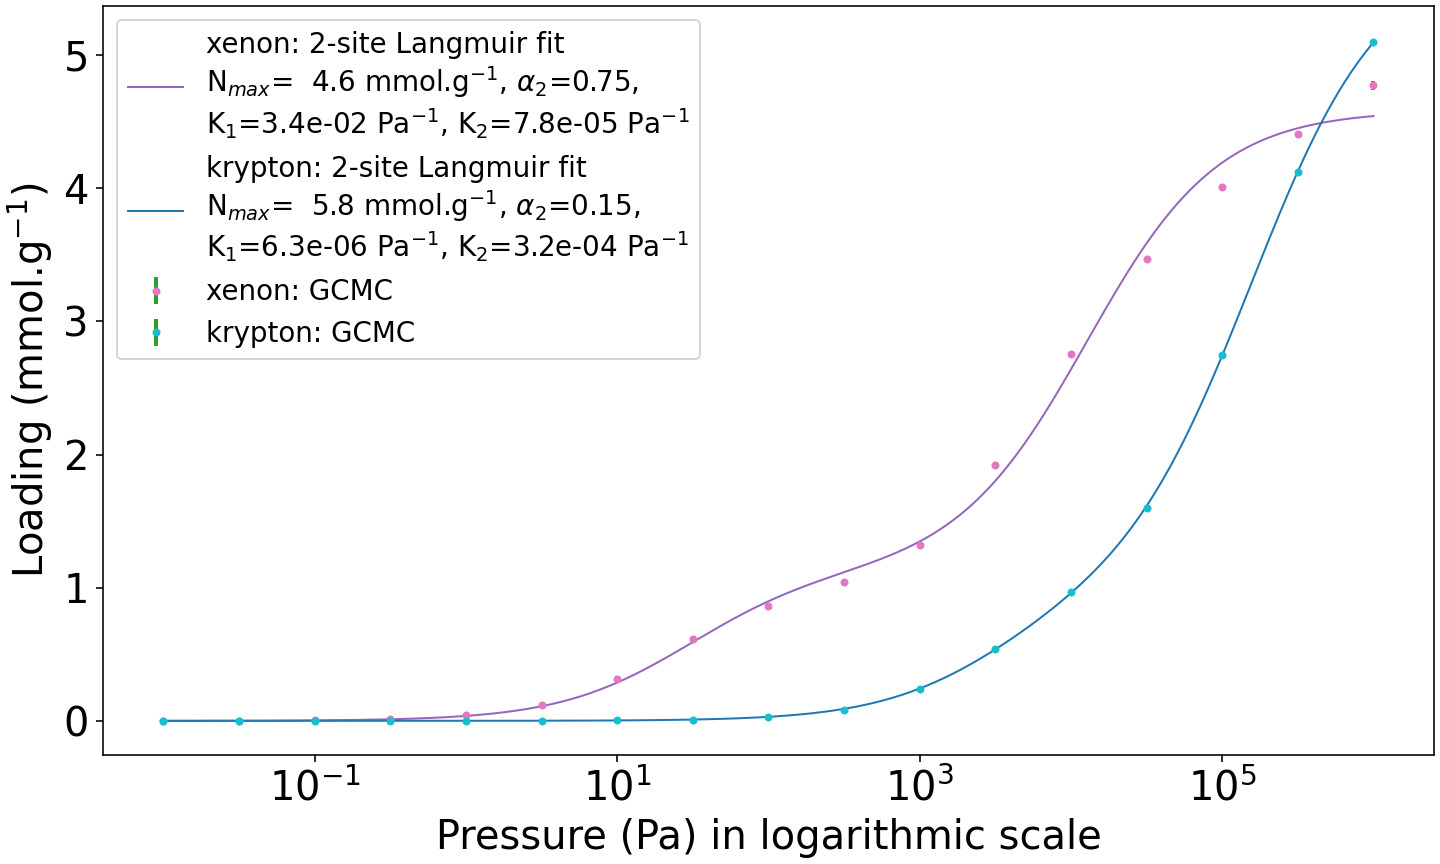
\includegraphics[width=0.4\textwidth]{figures/2-thermo/WOJJOV_clean_isotherm_xenon_krypton_298K.jpg}
  \caption{\small{\ WOJJOV : Représentation d'un MOF [Al(OH)(1,4-NDC)]$\cdot$2(H$_2$O) où NDC signifie naphthalenedicarboxylate. Code couleur : Cu en cyan foncé, C en gris, O en rouge, H en blanc ; Xe en rose et Kr en cyan clair. Sur la droite, les isothermes corps pur du xénon et krypton à \SI{298}{\kelvin} ainsi qu'un modèle d'isotherme à deux sites.}}
  \label{WOJJOV_resume}
\end{figure*}

Pour conclure, la présence de différents types de site et les réorganisations dues aux interactions du mélange Xe/Kr dans la phase d'adsorption permettent d'expliquer à l'échelle moléculaire la différence de sélectivité à basse et haute pression pour un certain nombre d'exemples. De plus, la séparation Xe/Kr est dominée par les effets enthalpiques, donc une bonne description de l'énergie d'adsorption est primordiale pour décrire la sélectivité d'un matériau.

\section*{Développement d'outils de criblage}

Dans un second temps, je me suis intéressée à différentes méthodes de calcul de l'enthalpie d'adsorption qui joue un rôle central dans la performance d'un matériau. Cette enthalpie à basse pression peut être théoriquement calculée grâce à un échantillonnage des énergies d'interaction pour tous les points accessibles de l'espace, mais cette méthode est coûteuse en temps de calcul. C'est pourquoi les méthodes d'échantillonnage aléatoire des points de l'espace se basant sur les algorithmes Monte Carlo sont plus souvent utilisées (insertion de Widom). Cependant, cet échantillonnage aléatoire ne tient donc pas en compte des informations que l'on a sur les matériaux nanoporeux. En effet, les adsorbats ne se situent pas à des endroits imprévisibles, ils sont souvent aux centres des pores (si la taille est adaptée) ou sur la surface des pores. On a donc exploité ces informations afin de diminuer le temps de calcul nécessaire à la détermination de l'enthalpie d'adsorption.

La première méthode approchée d'échantillonnage consiste à calculer les énergies sur les {n\oe{}uds} de Voronoï. Les n\oe{}uds de Voronoï sont des points équidistants à au moins quatre atomes de la structure. Si on considère uniquement les points de Voronoï accessibles, ces points seront situés au centre des pores. La deuxième méthode quant à elle échantillonne les surfaces des pores. Pour cela l'algorithme RAESS parcourt les points à la surface des atomes de la structure et y calcule l'énergie d'interaction avec le matériau. Et enfin, la dernière méthode développée durant cette thèse se base sur une grille symétrique optimisée pour faire baisser le temps de calcul par rapport à l'approche usuelle par grille. L'algorithme associé GrAED (\emph{Grid Adsorption Energy Descriptors}) est ainsi très intéressant pour des bases de données ayant des petits pores et des structures avec un haut degré de symétrie. La figure \ref{fgr:grid_perfomance_resume} compile les différentes performances de précision et de temps pour toutes les méthodes de calcul de l'enthalpie d'adsorption étudiée durant ma thèse.

\begin{figure}[ht]
\centering
    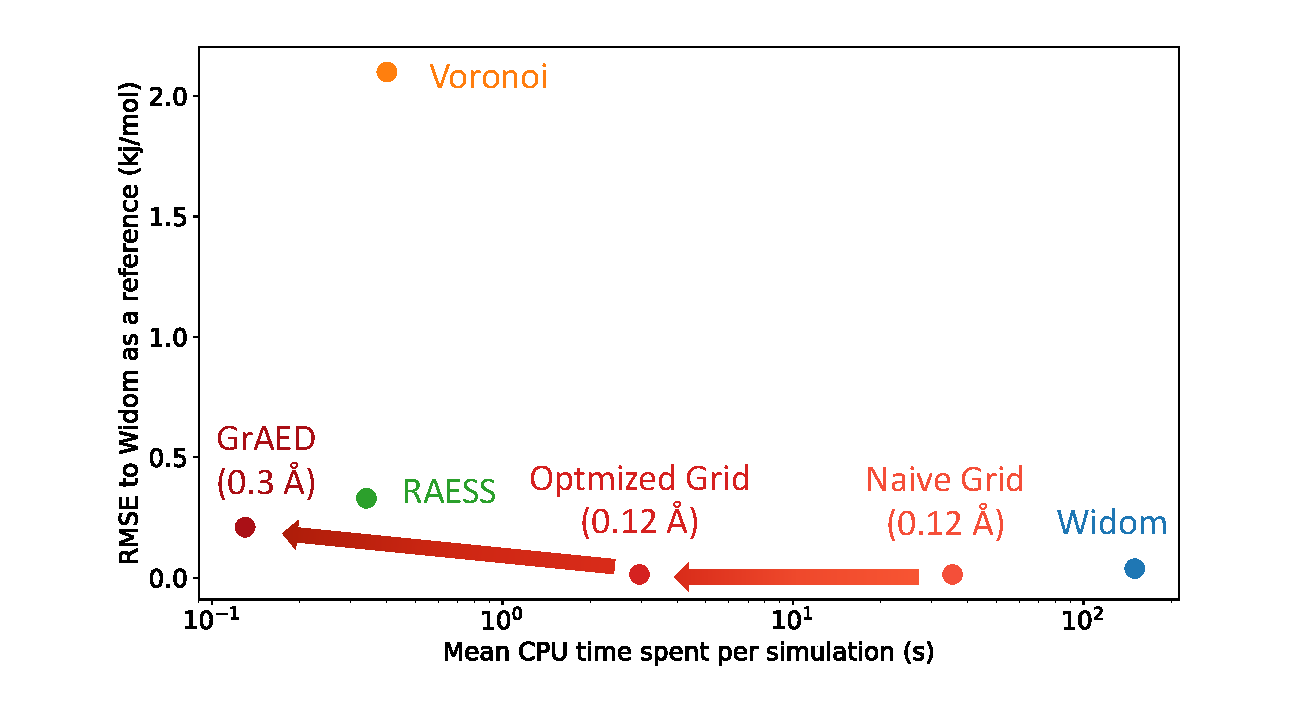
\includegraphics[width=0.7\textwidth]{figures/3-fastsim/Grid_sumup.pdf}
    \caption{Comparaison de la racine de l'erreur quadratique moyenne sur l'enthalpie d'adsorption du xénon et le temps de simulation par structure pour différentes méthodes d'échantillonnage  sur la base de données CoRE MOF 2019 (pour une taille de pore supérieure à \SI{3.7}{\angstrom}). }\label{fgr:grid_perfomance_resume}
\end{figure}

Pour développer une meilleure compréhension du processus de séparation, j'ai également développé un modèle de machine learning basé sur les descripteurs de GrAED et des descripteurs structurels plus couramment utilisés. Pour cela, la base de données CoRE MOF 2019 a été exploitée pour évaluer les valeurs de sélectivité en moins d'une minute, alors qu'une simulation de Monte Carlo grand canonique (GCMC) plus couramment utilisée requiert plus de \SI{40}{\minute}. 
Ce modèle donne de très bons résultats de prédiction tout en étant bien plus rapide que les simulations GCMC plus couramment utilisées. La figure~\ref{fgr:S1_prediction_resume} montre l'excellent accord entre les valeurs réelles et celles prédites par le modèle. Quantitativement, l'erreur sur le logarithme base 10 de la sélectivité vaut environ $0,06$ (RMSE), ce qui correspond à une excellente prédiction. 

\begin{figure}[h!]
\centering
    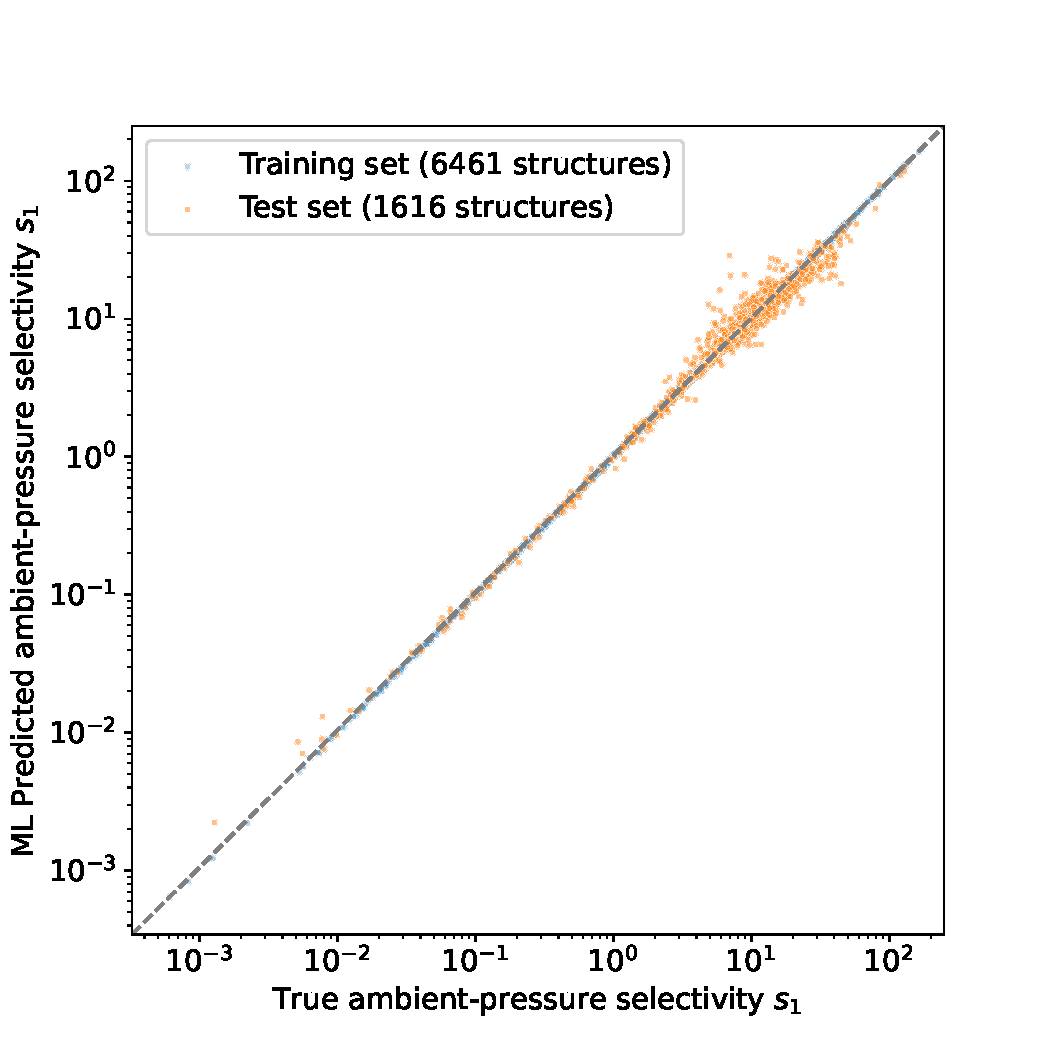
\includegraphics[width=0.48\linewidth]{figures/4-ml/SI_figure/Scatterplot_S1_prediction_logscale.pdf}
    \caption{Graphe de comparaison de la sélectivité Xe/Kr (à pression et température ambiantes pour une composition 20\pp{}80) prédite par le modèle et celle calculée par GCMC en échelle logarithmique. Les points colorés en bleu correspondent au jeu de données d'entraînement, tandis que ceux en orange correspondent au jeu de test. La superposition des points est faite de tel sort que l'on voit davantage les résultats sur le jeu de test pour évaluer la généralisabilité du modèle.}\label{fgr:S1_prediction_resume}
\end{figure}

Le second objectif de cette étude a été de mieux quantifier les origines de la différence observée entre la sélectivité à basse pression et celle à haute pression. Pour cela, le modèle ML a été interprété en utilisant des modèles d'interprétabilité comme les valeurs de Shapley. Ces résultats corroborent les deux causes principales attribuées d'une part à la diversité de taille et de nature des pores, et d'autre part à la réorganisation des adsorbats en espace confiné à la limite de la saturation des pores. Des facteurs quantitatifs expliquant ces changements de sélectivités ont ainsi été établis : les moyennes énergétiques à \SI{900}{\kelvin}, des mesures statistiques sur la diversité des énergies d'interaction, mais aussi des tailles de pore. 

Le modèle final peut ensuite être utilisé pour accélérer les méthodes de criblage actuelles. Par exemple, le criblage peut consister à mettre de côté des structures peu prometteuses en se basant sur des critères purement géométriques, puis des critères énergétiques calculés par l'algorithme de GrAED peuvent s'ajouter, pour enfin utiliser le modèle ML pour avoir une compréhension plus fine des performances de séparation. Cette méthode est pour l'instant testée et validée pour le cas de l'évaluation de la sélectivité Xe/Kr à pression ambiante, mais il peut s'étendre à des adsorbats d'une tout autre nature. 

Au-delà des effets purement thermodynamiques traités dans cette partie du résumé, mais aussi dans les chapitres 2, 3 et 4 de ma thèse, il existe également des effets cinétiques liés au transport des molécules d'adsorbat à l'intérieur des pores et des canaux du matériau.

\section*{Propriétés de transport}

Enfin, mes derniers travaux portent sur la modélisation des effets de transport du xénon et du krypton dans les structures poreuses de CoRE MOF 2019. Les effets de transport peuvent influencer les performances d'un matériau utilisé comme un adsorbant, comme illustré sur la figure~\ref{fgr:intro_diffusion_resume}. L'accès aux pores pour adsorption peut être plus ou moins rapide selon la vitesse de diffusion dans le matériau. Pour des membranes de séparation, l'effet de transport devient même la mesure principale de performance. Les effets de transport ont été estimés en utilisant des simulations de dynamique moléculaire.

\begin{figure}[ht]
    \centering
      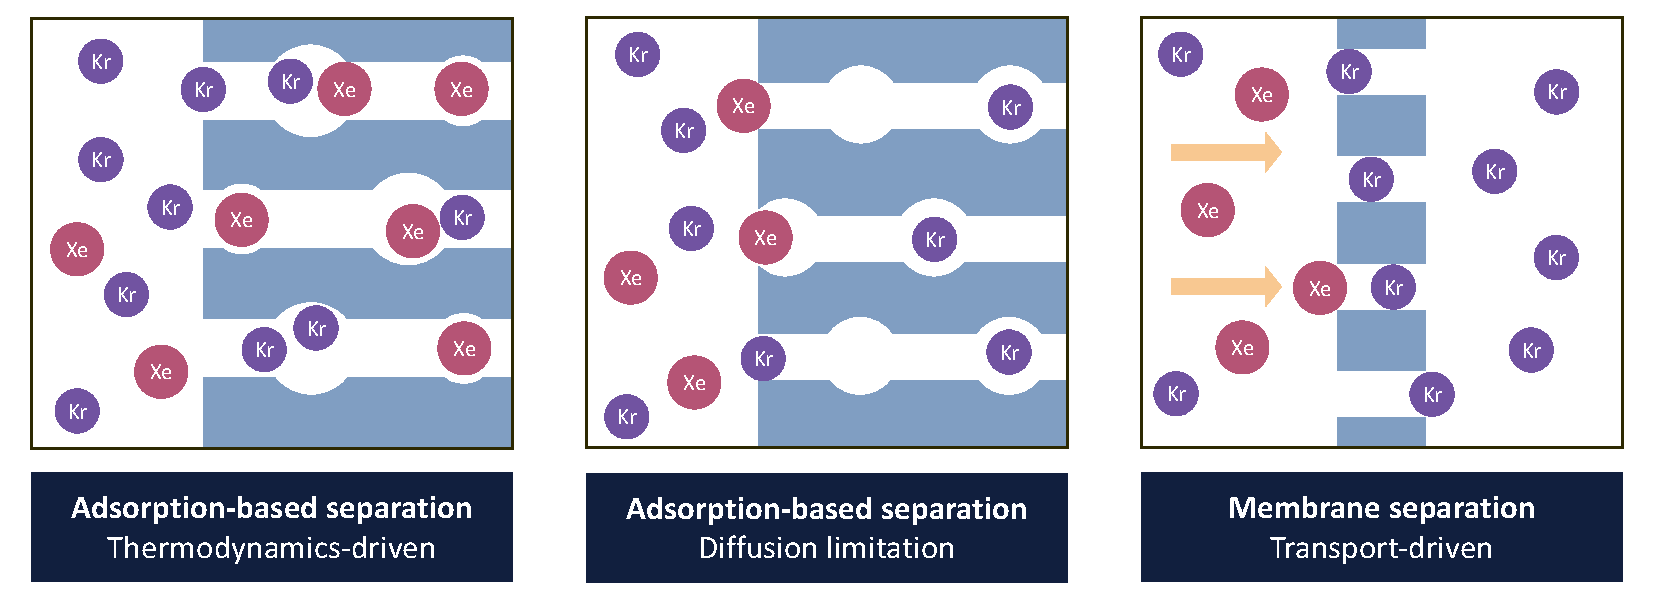
\includegraphics[width=0.95\textwidth]{figures/5-diffusion/Diffusion.pdf}
      \caption{Illustration of the comparative role of the thermodynamic and transport properties for Xe/Kr separation in nanoporous materials. From the transport dominated process of membrane separation to the thermodynamically equilibrated separation processes in the nanopores, different more nuanced cases could emerge where the diffusion imposes kinetic limitations.}\label{fgr:intro_diffusion_resume}
  \end{figure}

Dans cette étude, de nombreuses corrélations ont été analysées et deux descripteurs semblent expliquer les valeurs du coefficient de diffusion. En effet, le diamètre de la plus petite sphère pouvant diffuser librement dans les canaux du matériau (PLD), une caractéristique structurelle facilement calculable, semble corrélé au logarithme du coefficient de diffusion. On peut distinguer deux régimes sur la figure~\ref{fgr:barrier_diffusion_a_resume}: une relation plutôt linéaire suivie d'un plateau. 

Une mesure de la barrière énergétique de diffusion est également proposée en utilisant une grille calculée par l'algorithme GrAED. Cette barrière d'énergie semble inversement proportionnelle au logarithme du coefficient de diffusion comme on peut le voir sur la figure~\ref{fgr:barrier_diffusion_b_resume}. Cette corrélation n'est pas très forte avec un coefficient de Pearson de l'ordre de $-0.77$ si on considère toutes les structures. 

\begin{figure}[hb]
  \centering
  \begin{subfigure}[b]{0.48\textwidth}
      \centering
      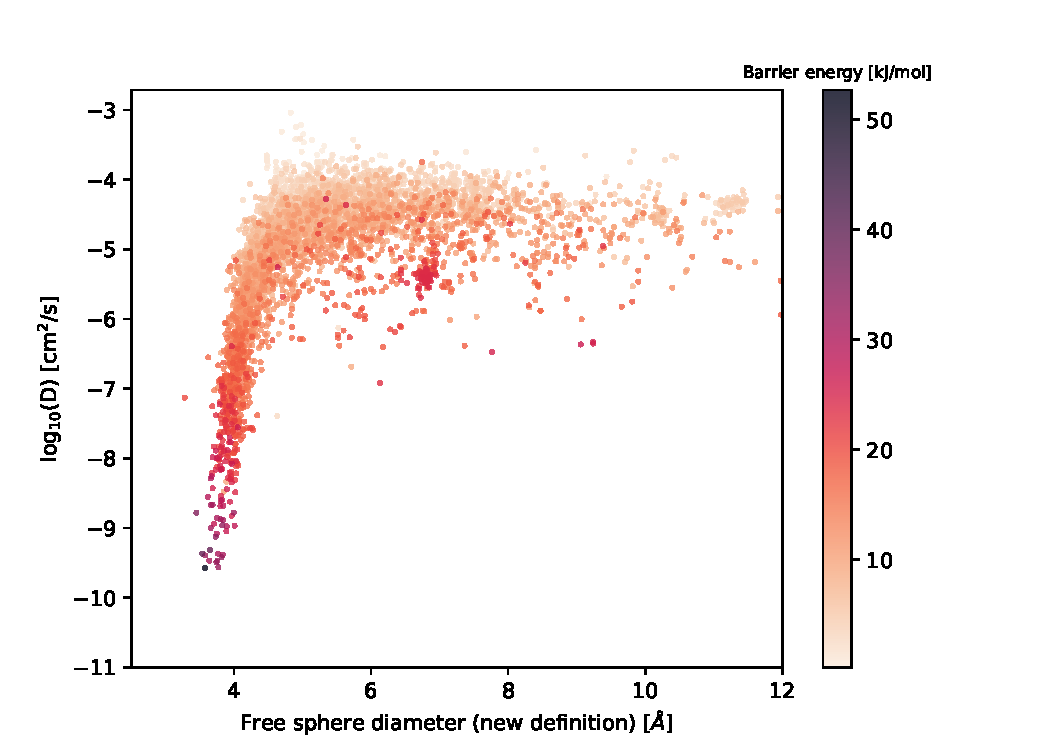
\includegraphics[width=\textwidth]{figures/5-diffusion/difflog_Df-uff298K_barrier.pdf}
      \caption{Taille caractéristique des canaux}\label{fgr:barrier_diffusion_a_resume}
  \end{subfigure}
  \hfill
  \begin{subfigure}[b]{0.48\textwidth}
      \centering
      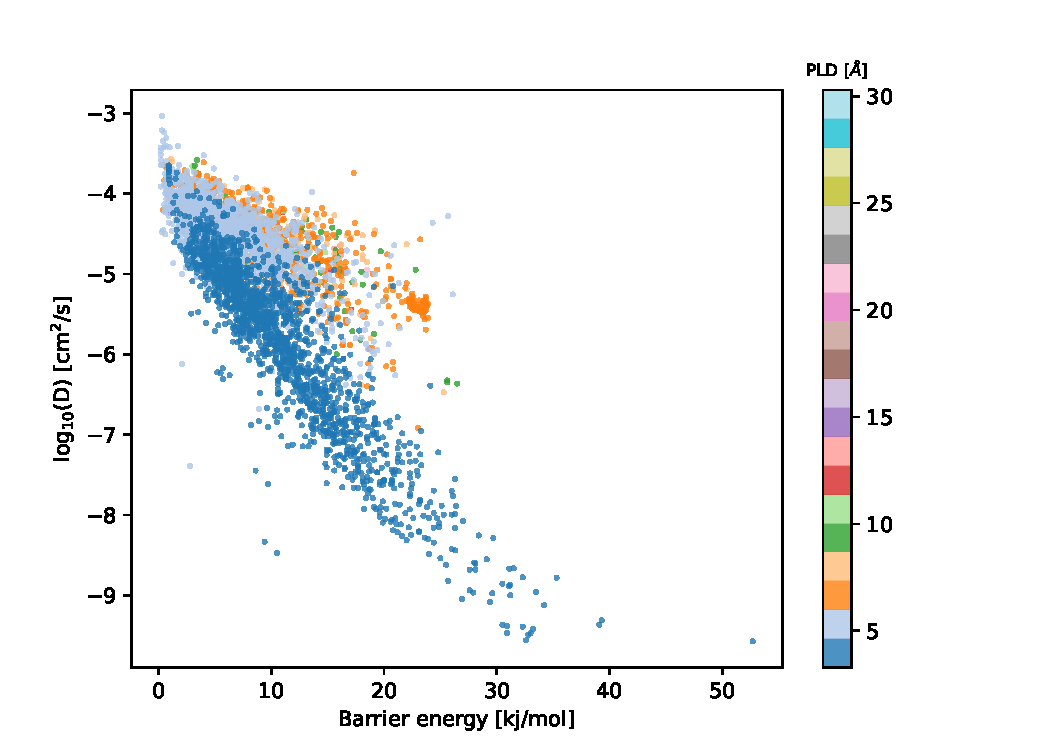
\includegraphics[width=\textwidth]{figures/5-diffusion/difflog_barrier_Df_uff.pdf}
      \caption{Barrière énergétique de diffusion}\label{fgr:barrier_diffusion_b_resume}
  \end{subfigure}
      \caption{ (a) Graphe comparant le logarithme base 10 du coefficient de diffusion du xénon à la taille des canaux mesurée par le diamètre minimal du canal (PLD, en anglais), et les points sont étiquetés par les énergies de barrière. (b) Graphe comparant le logarithme base 10 du coefficient de diffusion du xénon à la barrière énergétique de diffusion, les points sont étiquetés par le diamètre PLD. }\label{fgr:barrier_diffusion_resume}
  \end{figure}
  
En suivant une approche similaire à celle utilisée pour prédire la sélectivité, le logarithme du coefficient de coefficient du xénon a été prédit. Ce modèle se base notamment sur le diamètre PLD, la barrière énergétique et d'autres descripteurs thermodynamiques et structurels. Comme on peut le voir sur la figure~\ref{fgr:diff_pred_resume}, le modèle semble bien prédire l'ordre de grandeur du coefficient de diffusion du xénon avec une erreur de l'ordre de $0.25$ sur le $\log_{10}$ de ce coefficient. Cela signifie que l'on a une bonne connaissance de l'exposant du coefficient de diffusion exprimé comme une puissance de 10. Il est donc possible d'évaluer l'ordre de grandeur de la valeur du coefficient de diffusion tout en évitant des simulations de dynamique moléculaire requérant quelques jours de simulation.  

\begin{figure}[ht]
  \centering
  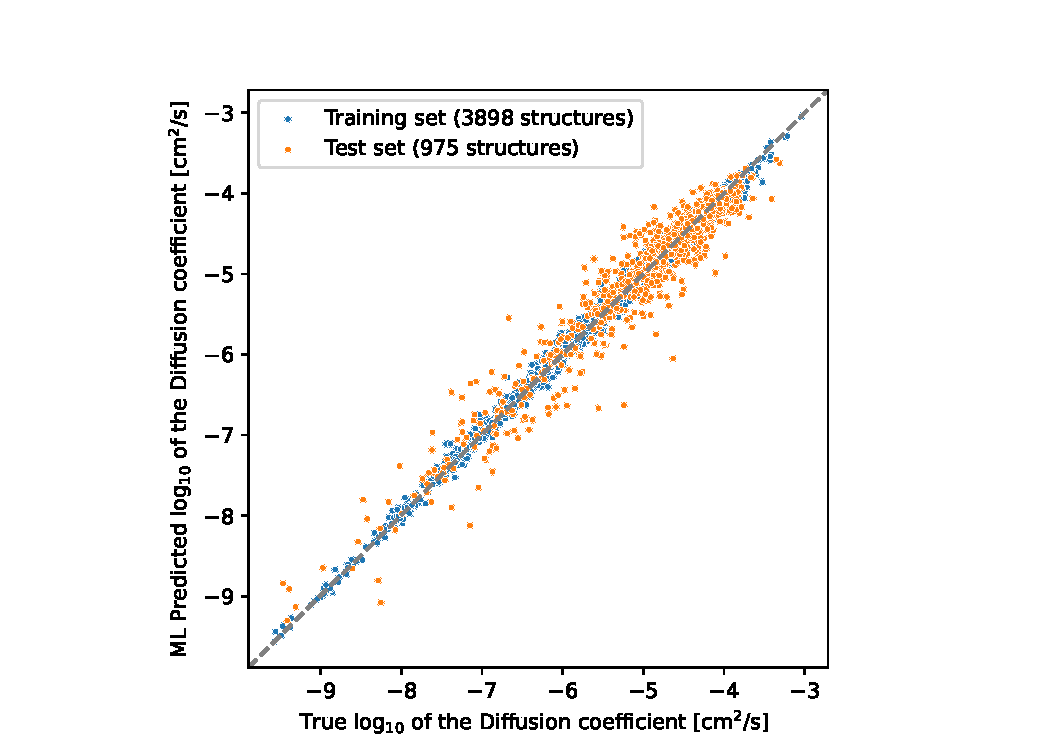
\includegraphics[width=0.5\textwidth]{figures/5-diffusion/diffusion_prediction.pdf}
  \caption{ Comparaison du $\log_{10}$ du coefficient de diffusion du xénon prédit par le modèle ML et les valeurs simulées par dynamique moléculaire. La racine de l'erreur quadratique moyenne sur le logarithme base 10 vaut $0.25$. }\label{fgr:diff_pred_resume}
\end{figure}


Ce modèle de machine learning permet ainsi de remplacer la méthode coûteuse de dynamique moléculaire par l'utilisation de simulations moins coûteuses (barrière d'énergie et descripteurs structurels). On peut appliquer cette méthode non seulement pour évaluer la cinétique de séparation dans un procédé de séparation par adsorption, mais il permet également de traiter d'autres cas d'application comme la sélectivité d'une membrane de séparation. Enfin, en comparant les rapports des coefficients de diffusion du xénon et du krypton aux valeurs de la sélectivité Xe/Kr, il est possible d'identifier de nouveaux matériaux qui ne présentent pas de blocage cinétique tout en ayant une sélectivité très importante.

D'autres méthodes basées sur la théorie des états de transition ont également été explorées pour calculer le coefficient de diffusion. Ces travaux ont notamment mené à la conception de l'algorithme utilisé pour calculer des barrières d'énergie. D'autres études sont encore nécessaires pour aller plus loin sur la description de la diffusion dans les canaux confinés des matériaux comme la prise en compte de la tortuosité, mais aussi la prise en compte des effets de diffusion collective où les équations de Fick et d'Eintein ne suffisent plus. 

\clearpage
\section*{Conclusion}

Cette thèse étudie ainsi les grandeurs thermodynamiques et cinétiques de la séparation xénon/krypton dans les matériaux nanoporeux. On a pu caractériser de manière plus fine les caractéristiques des matériaux les plus sélectifs. En ajoutant des contraintes sur la diffusibilité, différents types de matériaux ont été identifiés. 

La prise en compte de phénomènes physiques non inclus dans les études de cette thèse ouvre des perspectives pour de nombreux travaux sur ce sujet. En effet, de nouveaux travaux expérimentaux montrent l'importance de la prise en compte de la polarisation. Le matériau le plus sélectif à ce jour pour la séparation xénon/krypton se base sur l'interaction induite par des métaux non coordinés.\autocite{Pei_2022} Enfin, la flexibilité du matériau est également importante à prendre en compte. Dans certains cas, la flexibilité permet même de mieux comprendre l'incohérence entre les résultats expérimentaux et théoriques. De nombreuses pistes peuvent être explorées pour intégrer à l'avenir ces effets dans un criblage.\autocite{Lachet_1998,Witman_2017}

\vfill
\begin{center}
    \pgfornament[width=6cm,color=CTsemi]{75}
\end{center}
\vfill\vfill

\end{otherlanguage}

\OnlyInSubfile{\printglobalbibliography}

\end{document}
